%%%%%%%%%%%%%%%%%%%%%%%%%%%%%%%%%%%%%%%%%%%%%%%%%%%%%%%%%%%%%%%%%%%%%%%%%%%%%%%%%%%%%%%%%%%%%%%%%%%%%%%%%%%%%%%%%%%%%%%%%%%%%%%%%%%%%%%%%%%%%%%%%%%%%%%%%%%%%%%%%%%
% Written By Michael Brodskiy
% Class: Fundamentals of Electronics
% Professor: M. Onabajo
%%%%%%%%%%%%%%%%%%%%%%%%%%%%%%%%%%%%%%%%%%%%%%%%%%%%%%%%%%%%%%%%%%%%%%%%%%%%%%%%%%%%%%%%%%%%%%%%%%%%%%%%%%%%%%%%%%%%%%%%%%%%%%%%%%%%%%%%%%%%%%%%%%%%%%%%%%%%%%%%%%%

\documentclass[12pt]{article} 
\usepackage{alphalph}
\usepackage[utf8]{inputenc}
\usepackage[russian,english]{babel}
\usepackage{titling}
\usepackage{amsmath}
\usepackage{graphicx}
\usepackage{enumitem}
\usepackage{amssymb}
\usepackage[super]{nth}
\usepackage{everysel}
\usepackage{ragged2e}
\usepackage{geometry}
\usepackage{multicol}
\usepackage{fancyhdr}
\usepackage{cancel}
\usepackage{siunitx}
\usepackage{physics}
\usepackage{tikz}
\usepackage{mathdots}
\usepackage{yhmath}
\usepackage{cancel}
\usepackage{color}
\usepackage{array}
\usepackage{multirow}
\usepackage{gensymb}
\usepackage{tabularx}
\usepackage{extarrows}
\usepackage{booktabs}
\usepackage{lastpage}
\usetikzlibrary{fadings}
\usetikzlibrary{patterns}
\usetikzlibrary{shadows.blur}
\usetikzlibrary{shapes}

\geometry{top=1.0in,bottom=1.0in,left=1.0in,right=1.0in}
\newcommand{\subtitle}[1]{%
  \posttitle{%
    \par\end{center}
    \begin{center}\large#1\end{center}
    \vskip0.5em}%

}
\usepackage{hyperref}
\hypersetup{
colorlinks=true,
linkcolor=blue,
filecolor=magenta,      
urlcolor=blue,
citecolor=blue,
}


\title{Homework 7}
\date{\today}
\author{Michael Brodskiy\\ \small Professor: M. Onabajo}

\begin{document}

\maketitle

\begin{enumerate}

  \item We may begin by finding the DC equivalent by changing all capacitors to open circuits. This gets us:

    \begin{figure}[H]
      \centering
      \tikzset{every picture/.style={line width=0.75pt}} %set default line width to 0.75pt        

\begin{tikzpicture}[x=0.75pt,y=0.75pt,yscale=-1,xscale=1]
%uncomment if require: \path (0,590); %set diagram left start at 0, and has height of 590

%Straight Lines [id:da9680002872904098] 
\draw [line width=1.5]    (150,91.71) -- (150,83.29) ;
\draw [shift={(150,80.29)}, rotate = 90] [color={rgb, 255:red, 0; green, 0; blue, 0 }  ][line width=1.5]    (14.21,-4.28) .. controls (9.04,-1.82) and (4.3,-0.39) .. (0,0) .. controls (4.3,0.39) and (9.04,1.82) .. (14.21,4.28)   ;
%Shape: Resistor [id:dp8593801235190919] 
\draw   (150,111.13) -- (150,131.63) -- (161,136.18) -- (139,145.29) -- (161,154.4) -- (139,163.51) -- (161,172.62) -- (139,181.73) -- (161,190.84) -- (139,199.95) -- (150,204.5) -- (150,225) ;
%Straight Lines [id:da8544724471302622] 
\draw    (150,91.71) -- (150,111.13) ;
%Straight Lines [id:da8022666355674638] 
\draw    (236.42,225) -- (150,225) ;
%Shape: Resistor [id:dp8836502345629715] 
\draw   (150,225) -- (150,245.5) -- (161,250.05) -- (139,259.16) -- (161,268.27) -- (139,277.38) -- (161,286.49) -- (139,295.6) -- (161,304.71) -- (139,313.82) -- (150,318.37) -- (150,338.87) ;
%Straight Lines [id:da6300557445441965] 
\draw    (150,338.87) -- (150,358.29) ;
%Straight Lines [id:da4658089339797631] 
\draw    (160.71,361.29) -- (139.29,361.29) ;
%Straight Lines [id:da8064791145463434] 
\draw    (156.71,365.29) -- (144.29,365.29) ;
%Straight Lines [id:da23282831587418495] 
\draw    (152.71,369.29) -- (148.29,369.29) ;
%Shape: Resistor [id:dp17113966001084258] 
\draw   (251,249.42) -- (251,269.92) -- (262,274.47) -- (240,283.58) -- (262,292.69) -- (240,301.8) -- (262,310.91) -- (240,320.02) -- (262,329.13) -- (240,338.24) -- (251,342.79) -- (251,363.29) ;
%Straight Lines [id:da14398768168854004] 
\draw    (261.71,367.29) -- (240.29,367.29) ;
%Straight Lines [id:da889215723082148] 
\draw    (257.71,371.29) -- (245.29,371.29) ;
%Straight Lines [id:da5284581473425657] 
\draw    (253.71,375.29) -- (249.29,375.29) ;
%Shape: Circle [id:dp7771066805504848] 
\draw   (225.42,225) .. controls (225.42,211.19) and (236.61,200) .. (250.42,200) .. controls (264.23,200) and (275.42,211.19) .. (275.42,225) .. controls (275.42,238.81) and (264.23,250) .. (250.42,250) .. controls (236.61,250) and (225.42,238.81) .. (225.42,225) -- cycle ;
%Straight Lines [id:da8210220682512022] 
\draw [line width=1.5]    (236.42,225) -- (248.96,247.38) ;
\draw [shift={(250.42,250)}, rotate = 240.75] [color={rgb, 255:red, 0; green, 0; blue, 0 }  ][line width=1.5]    (14.21,-4.28) .. controls (9.04,-1.82) and (4.3,-0.39) .. (0,0) .. controls (4.3,0.39) and (9.04,1.82) .. (14.21,4.28)   ;
%Straight Lines [id:da37547982897555954] 
\draw    (236.42,235.71) -- (236.42,214.29) ;
%Straight Lines [id:da7596400997967242] 
\draw [line width=0.75]    (250.42,200) -- (236.42,225) ;
%Straight Lines [id:da04071305532058955] 
\draw    (250.42,200) -- (250.42,113.58) ;
%Straight Lines [id:da4395243182760231] 
\draw [line width=1.5]    (250.42,94.16) -- (250.42,85.74) ;
\draw [shift={(250.42,82.74)}, rotate = 90] [color={rgb, 255:red, 0; green, 0; blue, 0 }  ][line width=1.5]    (14.21,-4.28) .. controls (9.04,-1.82) and (4.3,-0.39) .. (0,0) .. controls (4.3,0.39) and (9.04,1.82) .. (14.21,4.28)   ;
%Straight Lines [id:da20933217115888925] 
\draw    (250.42,94.16) -- (250.42,113.58) ;

% Text Node
\draw (171,76.4) node [anchor=north west][inner sep=0.75pt]    {$+15\left[\text{V}\right]$};
% Text Node
\draw (163,157.8) node [anchor=north west][inner sep=0.75pt]    {$R_{1}$};
% Text Node
\draw (163,271.67) node [anchor=north west][inner sep=0.75pt]    {$R_{2}$};
% Text Node
\draw (264,277.87) node [anchor=north west][inner sep=0.75pt]    {$R_{E}$};


\end{tikzpicture}

      \caption{DC Equivalent Circuit}
      \label{fig:1}
    \end{figure}

    We can find a Th\'evenin equivalent for the $R_1$-$R_2$ voltage as:

    $$V_{th}=15\left[ \frac{10k}{10k+10k} \right]$$
    $$V_{th}=7.5[\si{\volt}]$$

    And then the equivalent resistance:

    $$R_{th}=\frac{10^2}{20}$$
    $$R_{th}=5[\si{\kilo\ohm}]$$

    This allows us to draw the circuit as:

    \begin{figure}[H]
      \centering
      \tikzset{every picture/.style={line width=0.75pt}} %set default line width to 0.75pt        

\begin{tikzpicture}[x=0.75pt,y=0.75pt,yscale=-1,xscale=1]
%uncomment if require: \path (0,590); %set diagram left start at 0, and has height of 590

%Straight Lines [id:da8022666355674638] 
\draw    (236.42,225) -- (225.42,225) ;
%Straight Lines [id:da6300557445441965] 
\draw    (111.55,347.84) -- (111.55,367.26) ;
%Straight Lines [id:da4658089339797631] 
\draw    (121.71,370.29) -- (100.29,370.29) ;
%Straight Lines [id:da8064791145463434] 
\draw    (117.71,374.29) -- (105.29,374.29) ;
%Straight Lines [id:da23282831587418495] 
\draw    (113.71,378.29) -- (109.29,378.29) ;
%Shape: Resistor [id:dp17113966001084258] 
\draw   (251,249.42) -- (251,269.92) -- (262,274.47) -- (240,283.58) -- (262,292.69) -- (240,301.8) -- (262,310.91) -- (240,320.02) -- (262,329.13) -- (240,338.24) -- (251,342.79) -- (251,363.29) ;
%Straight Lines [id:da14398768168854004] 
\draw    (261.71,367.29) -- (240.29,367.29) ;
%Straight Lines [id:da889215723082148] 
\draw    (257.71,371.29) -- (245.29,371.29) ;
%Straight Lines [id:da5284581473425657] 
\draw    (253.71,375.29) -- (249.29,375.29) ;
%Shape: Circle [id:dp7771066805504848] 
\draw   (225.42,225) .. controls (225.42,211.19) and (236.61,200) .. (250.42,200) .. controls (264.23,200) and (275.42,211.19) .. (275.42,225) .. controls (275.42,238.81) and (264.23,250) .. (250.42,250) .. controls (236.61,250) and (225.42,238.81) .. (225.42,225) -- cycle ;
%Straight Lines [id:da8210220682512022] 
\draw [line width=1.5]    (236.42,225) -- (248.96,247.38) ;
\draw [shift={(250.42,250)}, rotate = 240.75] [color={rgb, 255:red, 0; green, 0; blue, 0 }  ][line width=1.5]    (14.21,-4.28) .. controls (9.04,-1.82) and (4.3,-0.39) .. (0,0) .. controls (4.3,0.39) and (9.04,1.82) .. (14.21,4.28)   ;
%Straight Lines [id:da37547982897555954] 
\draw    (236.42,235.71) -- (236.42,214.29) ;
%Straight Lines [id:da7596400997967242] 
\draw [line width=0.75]    (250.42,200) -- (236.42,225) ;
%Straight Lines [id:da04071305532058955] 
\draw    (250.42,200) -- (250.42,113.58) ;
%Straight Lines [id:da4395243182760231] 
\draw [line width=1.5]    (250.42,94.16) -- (250.42,85.74) ;
\draw [shift={(250.42,82.74)}, rotate = 90] [color={rgb, 255:red, 0; green, 0; blue, 0 }  ][line width=1.5]    (14.21,-4.28) .. controls (9.04,-1.82) and (4.3,-0.39) .. (0,0) .. controls (4.3,0.39) and (9.04,1.82) .. (14.21,4.28)   ;
%Straight Lines [id:da20933217115888925] 
\draw    (250.42,94.16) -- (250.42,113.58) ;
%Shape: Resistor [id:dp6505678637158546] 
\draw   (111.55,225) -- (132.05,225) -- (136.6,214) -- (145.71,236) -- (154.82,214) -- (163.93,236) -- (173.04,214) -- (182.15,236) -- (191.26,214) -- (200.37,236) -- (204.93,225) -- (225.42,225) ;
%Shape: Circle [id:dp39982521241705204] 
\draw   (86.55,286.42) .. controls (86.55,272.61) and (97.75,261.42) .. (111.55,261.42) .. controls (125.36,261.42) and (136.55,272.61) .. (136.55,286.42) .. controls (136.55,300.23) and (125.36,311.42) .. (111.55,311.42) .. controls (97.75,311.42) and (86.55,300.23) .. (86.55,286.42) -- cycle ;
%Straight Lines [id:da328306748259789] 
\draw    (111.55,261.42) -- (111.55,225) ;
%Straight Lines [id:da8390625705334938] 
\draw    (111.55,347.84) -- (111.55,311.42) ;

% Text Node
\draw (252.42,79.34) node [anchor=south west] [inner sep=0.75pt]    {$+15\left[\text{V}\right]$};
% Text Node
\draw (264,277.87) node [anchor=north west][inner sep=0.75pt]    {$R_{E}$};
% Text Node
\draw (111.55,286.42) node    {$V_{th}$};
% Text Node
\draw (111.55,261.82) node [anchor=north] [inner sep=0.75pt]    {$+$};
% Text Node
\draw (111.55,308.02) node [anchor=south] [inner sep=0.75pt]    {$-$};
% Text Node
\draw (165.93,239.4) node [anchor=north west][inner sep=0.75pt]    {$R_{th}$};


\end{tikzpicture}

      \caption{DC Equivalent Simplified}
      \label{fig:2}
    \end{figure}

    We use KVL at the base-emitter loop to getL

    $$-V_{th}+I_BR_{th}+V_{BE}+I_{E}R_E=0$$

    Since we know $I_E=(1+\beta)I_B$, we may write:

    $$-V_{th}+I_BR_{th}+V_{BE}+(1+\beta)I_BR_E=0$$

    Rearranging, we get:

    $$I_B=\frac{V_{th}-V_{BE}}{R_{th}+(1+\beta)R_E}$$

    We plug in our known values to get:

    $$I_B=\frac{7.5-.7}{5k+(1+100)1k}$$
    $$I_B=64.151[\si{\micro\ampere}]$$

    From this, we may find:

    $$I_{CQ}=\beta I_B$$
    $$I_{CQ}=(100)(64.151\cdot10^{-6})$$
    $$\boxed{I_{CQ}=6.4151[\si{\milli\ampere}]}$$

    We can find $r_{\pi}$ by using the equation:

    $$r_{\pi}=\frac{\beta}{g_m}$$

    Where $g_m=\dfrac{I_{CQ}}{V_T}$:

    $$r_{\pi}=\frac{\beta V_T}{I_{CQ}}$$
    $$r_{\pi}=\frac{100(.026)}{.0064151}$$
    $$\boxed{r_{\pi}=405.29[\si{\ohm}]}$$

    We can then perform a small-signal analysis by finding $r_e$:

    $$r_e=\frac{\beta V_T}{(1+\beta)I_{CQ}}$$
    $$r_e=4.0128[\si{\ohm}]$$

    Using this, we can use our small-signal analysis model to find the gain. First, we get:

    $$V_o=V_i\left[ \frac{R_ER_L}{(R_E+R_L)r_e+R_ER_L} \right]$$

    Thus, we see that the voltage gain is:

    $$A_v=\left[ \frac{R_ER_L}{(R_E+R_L)r_e+R_ER_L} \right]$$

    We plug in our known values to find:

    $$A_v=\left[ \frac{(1000)(500)}{(1500)(4.0128)+(500000)} \right]$$
    $$\boxed{A_v=.9881}$$

    Furthermore, we can find the open-loop voltage gain when $R_L\to\infty$:

    $$A_{voc}=\left[ \frac{R_E}{r_e+R_E} \right]$$
    $$A_{voc}=\left[ \frac{1000}{4.0128+1000} \right]$$
    $$\boxed{A_{voc}=.996}$$

    Now, we can work to find the input impedance. First and foremost, we know:

    $$i_e=V_i\left[ \frac{R_ER_L}{(R_E+R_L)r_e+R_ER_L} \right]$$

    Using KCL for the input current node, we may observe:

    $$i_i+\frac{\beta}{\beta+1}i_e=V_i\left[ \frac{R_1+R_2}{R_1R_2} \right]+i_e$$

    We can rearrange this to find:

    $$\frac{V_i}{i_i}=\left[ \frac{R_1+R_2}{R_1R_2}+\frac{R_E+R_L}{(1+\beta)[(R_E+R_L)r_e+R_ER_L]} \right]^{-1}$$
    $$Z_{i}=\left(2.2935\cdot10^{-4}\right)^{-1}$$
    $$\boxed{Z_{i}=4360.2[\si{\ohm}]}$$

    The current gain may be expressed as the ratio of input ($Z_i$) and output ($R_L$) impedances:

    $$A_i=A_v\frac{Z_i}{R_L}$$
    $$\boxed{A_i=8.6854}$$

    From here, we know the power gain is:

    $$G=A_iA_v$$
    $$G=(.996)(8.6854)$$
    $$\boxed{G=8.6507}$$

    Finally, we can find the output resistant by computing several parallel resistances:

    $$Z_o=R_E||\left[ \frac{R_B||R_S+r_{\pi}}{\beta +1} \right]$$

    We plug in known values:

    $$Z_o=1k||\left[ \frac{833+405.29}{101} \right]$$
    $$Z_o=1k||12.264$$
    $$\boxed{Z_o=12.115[\si{\ohm}]}$$

  \item

    We begin by investigating $V_{hum}\to 0$, which shows that the circuit is the same for both figures:

    \begin{figure}[H]
      \centering
      \tikzset{every picture/.style={line width=0.75pt}} %set default line width to 0.75pt        

\begin{tikzpicture}[x=0.75pt,y=0.75pt,yscale=-1,xscale=1]
%uncomment if require: \path (0,590); %set diagram left start at 0, and has height of 590

%Straight Lines [id:da6300557445441965] 
\draw    (122.55,346.84) -- (122.55,366.26) ;
%Straight Lines [id:da4658089339797631] 
\draw    (132.71,369.29) -- (111.29,369.29) ;
%Straight Lines [id:da8064791145463434] 
\draw    (128.71,373.29) -- (116.29,373.29) ;
%Straight Lines [id:da23282831587418495] 
\draw    (124.71,377.29) -- (120.29,377.29) ;
%Shape: Resistor [id:dp17113966001084258] 
\draw   (196,249.42) -- (196,269.92) -- (207,274.47) -- (185,283.58) -- (207,292.69) -- (185,301.8) -- (207,310.91) -- (185,320.02) -- (207,329.13) -- (185,338.24) -- (196,342.79) -- (196,363.29) ;
%Straight Lines [id:da14398768168854004] 
\draw    (206.71,367.29) -- (185.29,367.29) ;
%Straight Lines [id:da889215723082148] 
\draw    (202.71,371.29) -- (190.29,371.29) ;
%Straight Lines [id:da5284581473425657] 
\draw    (198.71,375.29) -- (194.29,375.29) ;
%Shape: Circle [id:dp39982521241705204] 
\draw   (97.55,286.42) .. controls (97.55,272.61) and (108.75,261.42) .. (122.55,261.42) .. controls (136.36,261.42) and (147.55,272.61) .. (147.55,286.42) .. controls (147.55,300.23) and (136.36,311.42) .. (122.55,311.42) .. controls (108.75,311.42) and (97.55,300.23) .. (97.55,286.42) -- cycle ;
%Straight Lines [id:da328306748259789] 
\draw    (122.13,261.42) -- (122.13,225) ;
%Straight Lines [id:da8390625705334938] 
\draw    (122.55,347.84) -- (122.55,311.42) ;
%Straight Lines [id:da5265252364443316] 
\draw    (196,249.42) -- (195.97,227) ;
%Shape: Resistor [id:dp14261323732847786] 
\draw   (268,251.42) -- (268,271.92) -- (279,276.47) -- (257,285.58) -- (279,294.69) -- (257,303.8) -- (279,312.91) -- (257,322.02) -- (279,331.13) -- (257,340.24) -- (268,344.79) -- (268,365.29) ;
%Straight Lines [id:da5402401224515765] 
\draw    (314.71,391.29) -- (293.29,391.29) ;
%Straight Lines [id:da8198849685910031] 
\draw    (310.71,395.29) -- (298.29,395.29) ;
%Straight Lines [id:da9139033536127192] 
\draw    (306.71,399.29) -- (302.29,399.29) ;
%Straight Lines [id:da48142531835954605] 
\draw    (195.55,227) -- (268.97,229) ;
%Straight Lines [id:da5655907469699456] 
\draw    (268,251.42) -- (267.97,229) ;
%Straight Lines [id:da2990554002516722] 
\draw    (304.74,388.71) -- (304.71,366.29) ;
%Straight Lines [id:da4284706467797289] 
\draw    (122.13,225) -- (195.55,227) ;
%Straight Lines [id:da41932097427349446] 
\draw    (268,365.29) -- (341.42,367.29) ;
%Shape: Diamond [id:dp5349776092477291] 
\draw   (341.4,274.87) -- (366.9,309.87) -- (341.4,344.87) -- (315.9,309.87) -- cycle ;
%Straight Lines [id:da8080706621300265] 
\draw    (341.42,367.29) -- (341.4,344.87) ;
%Straight Lines [id:da9678193687612239] 
\draw [line width=1.5]    (341.4,325.87) -- (341.4,289.87) ;
\draw [shift={(341.4,329.87)}, rotate = 270] [fill={rgb, 255:red, 0; green, 0; blue, 0 }  ][line width=0.08]  [draw opacity=0] (11.61,-5.58) -- (0,0) -- (11.61,5.58) -- cycle    ;
%Straight Lines [id:da18296338023582348] 
\draw    (341.4,274.87) -- (341.4,231) ;
%Straight Lines [id:da27786988283663827] 
\draw    (341.4,231) -- (413.82,233) ;
%Shape: Resistor [id:dp47531255017629714] 
\draw   (413,255.42) -- (413,275.92) -- (424,280.47) -- (402,289.58) -- (424,298.69) -- (402,307.8) -- (424,316.91) -- (402,326.02) -- (424,335.13) -- (402,344.24) -- (413,348.79) -- (413,369.29) ;
%Straight Lines [id:da006113327463057039] 
\draw    (423.71,373.29) -- (402.29,373.29) ;
%Straight Lines [id:da8707380132685233] 
\draw    (419.71,377.29) -- (407.29,377.29) ;
%Straight Lines [id:da31545889187691845] 
\draw    (415.71,381.29) -- (411.29,381.29) ;
%Straight Lines [id:da5875228315528056] 
\draw    (413,255.42) -- (412.97,233) ;
%Straight Lines [id:da5804304305948264] 
\draw    (413.82,233) -- (483.89,234.94) ;
\draw [shift={(486.24,235)}, rotate = 1.58] [color={rgb, 255:red, 0; green, 0; blue, 0 }  ][line width=0.75]      (0, 0) circle [x radius= 3.35, y radius= 3.35]   ;
%Straight Lines [id:da7683972867416118] 
\draw    (265.98,220.94) -- (195.55,219) ;
\draw [shift={(267.97,221)}, rotate = 181.58] [color={rgb, 255:red, 0; green, 0; blue, 0 }  ][line width=0.75]    (10.93,-3.29) .. controls (6.95,-1.4) and (3.31,-0.3) .. (0,0) .. controls (3.31,0.3) and (6.95,1.4) .. (10.93,3.29)   ;

% Text Node
\draw (209,277.87) node [anchor=north west][inner sep=0.75pt]    {$R_{B}$};
% Text Node
\draw (122.55,286.42) node    {$V_{in}$};
% Text Node
\draw (122.55,261.82) node [anchor=north] [inner sep=0.75pt]    {$+$};
% Text Node
\draw (122.55,308.02) node [anchor=south] [inner sep=0.75pt]    {$-$};
% Text Node
\draw (281,279.87) node [anchor=north west][inner sep=0.75pt]    {$r_{\pi }$};
% Text Node
\draw (368.9,309.87) node [anchor=west] [inner sep=0.75pt]    {$\beta I_{B}$};
% Text Node
\draw (426,283.87) node [anchor=north west][inner sep=0.75pt]    {$R_{C}$};
% Text Node
\draw (488.24,238.4) node [anchor=north west][inner sep=0.75pt]    {$V_{o}$};
% Text Node
\draw (269.97,217.6) node [anchor=south west] [inner sep=0.75pt]    {$I_{B}$};


\end{tikzpicture}

      \caption{Equivalent Circuit is the Same for $V_{hum}\to0$}
      \label{fig:3}
    \end{figure}

    From this, we may observe that:

    $$\boxed{A_v\approx -\frac{\beta R_C}{r_{\pi}}}$$

    We can then investigate the case when $V_{hum}\neq 0$ and $V_{in}\to0$. For the first figure, we see:

    \begin{figure}[H]
      \centering
      \tikzset{every picture/.style={line width=0.75pt}} %set default line width to 0.75pt        

\begin{tikzpicture}[x=0.75pt,y=0.75pt,yscale=-1,xscale=1]
%uncomment if require: \path (0,590); %set diagram left start at 0, and has height of 590

%Straight Lines [id:da6300557445441965] 
\draw    (122.55,346.84) -- (122.55,366.26) ;
%Straight Lines [id:da4658089339797631] 
\draw    (132.71,369.29) -- (111.29,369.29) ;
%Straight Lines [id:da8064791145463434] 
\draw    (128.71,373.29) -- (116.29,373.29) ;
%Straight Lines [id:da23282831587418495] 
\draw    (124.71,377.29) -- (120.29,377.29) ;
%Shape: Resistor [id:dp17113966001084258] 
\draw   (196,249.42) -- (196,269.92) -- (207,274.47) -- (185,283.58) -- (207,292.69) -- (185,301.8) -- (207,310.91) -- (185,320.02) -- (207,329.13) -- (185,338.24) -- (196,342.79) -- (196,363.29) ;
%Straight Lines [id:da14398768168854004] 
\draw    (206.71,367.29) -- (185.29,367.29) ;
%Straight Lines [id:da889215723082148] 
\draw    (202.71,371.29) -- (190.29,371.29) ;
%Straight Lines [id:da5284581473425657] 
\draw    (198.71,375.29) -- (194.29,375.29) ;
%Straight Lines [id:da328306748259789] 
\draw    (122.55,346.84) -- (122.13,225) ;
%Straight Lines [id:da5265252364443316] 
\draw    (196,249.42) -- (195.97,227) ;
%Shape: Resistor [id:dp14261323732847786] 
\draw   (268,251.42) -- (268,271.92) -- (279,276.47) -- (257,285.58) -- (279,294.69) -- (257,303.8) -- (279,312.91) -- (257,322.02) -- (279,331.13) -- (257,340.24) -- (268,344.79) -- (268,365.29) ;
%Straight Lines [id:da5402401224515765] 
\draw    (314.71,464.29) -- (293.29,464.29) ;
%Straight Lines [id:da8198849685910031] 
\draw    (310.71,468.29) -- (298.29,468.29) ;
%Straight Lines [id:da9139033536127192] 
\draw    (306.71,472.29) -- (302.29,472.29) ;
%Straight Lines [id:da48142531835954605] 
\draw    (195.55,227) -- (268.97,229) ;
%Straight Lines [id:da5655907469699456] 
\draw    (268,251.42) -- (267.97,229) ;
%Straight Lines [id:da2990554002516722] 
\draw    (304.74,388.71) -- (304.71,366.29) ;
%Straight Lines [id:da4284706467797289] 
\draw    (122.13,225) -- (195.55,227) ;
%Straight Lines [id:da41932097427349446] 
\draw    (268,365.29) -- (341.42,367.29) ;
%Shape: Diamond [id:dp5349776092477291] 
\draw   (341.4,274.87) -- (366.9,309.87) -- (341.4,344.87) -- (315.9,309.87) -- cycle ;
%Straight Lines [id:da8080706621300265] 
\draw    (341.42,367.29) -- (341.4,344.87) ;
%Straight Lines [id:da9678193687612239] 
\draw [line width=1.5]    (341.4,325.87) -- (341.4,289.87) ;
\draw [shift={(341.4,329.87)}, rotate = 270] [fill={rgb, 255:red, 0; green, 0; blue, 0 }  ][line width=0.08]  [draw opacity=0] (11.61,-5.58) -- (0,0) -- (11.61,5.58) -- cycle    ;
%Straight Lines [id:da18296338023582348] 
\draw    (341.4,274.87) -- (341.4,231) ;
%Straight Lines [id:da27786988283663827] 
\draw    (341.4,231) -- (413.82,233) ;
%Shape: Resistor [id:dp47531255017629714] 
\draw   (413,255.42) -- (413,275.92) -- (424,280.47) -- (402,289.58) -- (424,298.69) -- (402,307.8) -- (424,316.91) -- (402,326.02) -- (424,335.13) -- (402,344.24) -- (413,348.79) -- (413,369.29) ;
%Straight Lines [id:da006113327463057039] 
\draw    (423.71,373.29) -- (402.29,373.29) ;
%Straight Lines [id:da8707380132685233] 
\draw    (419.71,377.29) -- (407.29,377.29) ;
%Straight Lines [id:da31545889187691845] 
\draw    (415.71,381.29) -- (411.29,381.29) ;
%Straight Lines [id:da5875228315528056] 
\draw    (413,255.42) -- (412.97,233) ;
%Straight Lines [id:da5804304305948264] 
\draw    (413.82,233) -- (483.89,234.94) ;
\draw [shift={(486.24,235)}, rotate = 1.58] [color={rgb, 255:red, 0; green, 0; blue, 0 }  ][line width=0.75]      (0, 0) circle [x radius= 3.35, y radius= 3.35]   ;
%Straight Lines [id:da7683972867416118] 
\draw    (265.98,220.94) -- (195.55,219) ;
\draw [shift={(267.97,221)}, rotate = 181.58] [color={rgb, 255:red, 0; green, 0; blue, 0 }  ][line width=0.75]    (10.93,-3.29) .. controls (6.95,-1.4) and (3.31,-0.3) .. (0,0) .. controls (3.31,0.3) and (6.95,1.4) .. (10.93,3.29)   ;
%Shape: Circle [id:dp6906017931984727] 
\draw   (279.55,413.42) .. controls (279.55,399.61) and (290.75,388.42) .. (304.55,388.42) .. controls (318.36,388.42) and (329.55,399.61) .. (329.55,413.42) .. controls (329.55,427.23) and (318.36,438.42) .. (304.55,438.42) .. controls (290.75,438.42) and (279.55,427.23) .. (279.55,413.42) -- cycle ;
%Straight Lines [id:da0846557684176299] 
\draw    (304.58,460.84) -- (304.55,438.42) ;

% Text Node
\draw (209,277.87) node [anchor=north west][inner sep=0.75pt]    {$R_{B}$};
% Text Node
\draw (281,279.87) node [anchor=north west][inner sep=0.75pt]    {$r_{\pi }$};
% Text Node
\draw (368.9,309.87) node [anchor=west] [inner sep=0.75pt]    {$\beta I_{B}$};
% Text Node
\draw (426,283.87) node [anchor=north west][inner sep=0.75pt]    {$R_{C}$};
% Text Node
\draw (488.24,238.4) node [anchor=north west][inner sep=0.75pt]    {$V_{o}$};
% Text Node
\draw (269.97,217.6) node [anchor=south west] [inner sep=0.75pt]    {$I_{B}$};
% Text Node
\draw (304.55,413.42) node    {$V_{hum}$};
% Text Node
\draw (304.55,388.82) node [anchor=north] [inner sep=0.75pt]    {$+$};
% Text Node
\draw (304.55,435.02) node [anchor=south] [inner sep=0.75pt]    {$-$};
% Text Node
\draw (120.13,228.4) node [anchor=north east] [inner sep=0.75pt]    {$V_{in}\rightarrow 0$};


\end{tikzpicture}

      \caption{Equivalent Circuit for Figure (a) as $V_{in}\to0$}
      \label{fig:4}
    \end{figure}

    We may conclude that the hum gain can be expressed as:

    $$\boxed{A_{(a)}=\frac{\beta R_C}{r_{\pi}}}$$

    Finally, we may draw the equivalent circuit for the second figure to get:

    \begin{figure}[H]
      \centering
      \tikzset{every picture/.style={line width=0.75pt}} %set default line width to 0.75pt        

\begin{tikzpicture}[x=0.75pt,y=0.75pt,yscale=-1,xscale=1]
%uncomment if require: \path (0,590); %set diagram left start at 0, and has height of 590

%Straight Lines [id:da6300557445441965] 
\draw    (122.55,346.84) -- (122.55,366.26) ;
%Straight Lines [id:da4658089339797631] 
\draw    (132.71,369.29) -- (111.29,369.29) ;
%Straight Lines [id:da8064791145463434] 
\draw    (128.71,373.29) -- (116.29,373.29) ;
%Straight Lines [id:da23282831587418495] 
\draw    (124.71,377.29) -- (120.29,377.29) ;
%Shape: Resistor [id:dp17113966001084258] 
\draw   (292.48,165) -- (312.97,165) -- (317.53,154) -- (326.64,176) -- (335.75,154) -- (344.86,176) -- (353.97,154) -- (363.08,176) -- (372.19,154) -- (381.3,176) -- (385.85,165) -- (406.35,165) ;
%Straight Lines [id:da328306748259789] 
\draw    (122.13,261.42) -- (122.13,225) ;
%Straight Lines [id:da8390625705334938] 
\draw    (122.55,347.84) -- (122.13,261.42) ;
%Straight Lines [id:da5265252364443316] 
\draw    (170.55,227) -- (170.53,163.58) ;
%Shape: Resistor [id:dp14261323732847786] 
\draw   (268,251.42) -- (268,271.92) -- (279,276.47) -- (257,285.58) -- (279,294.69) -- (257,303.8) -- (279,312.91) -- (257,322.02) -- (279,331.13) -- (257,340.24) -- (268,344.79) -- (268,365.29) ;
%Straight Lines [id:da5402401224515765] 
\draw    (314.71,391.29) -- (293.29,391.29) ;
%Straight Lines [id:da8198849685910031] 
\draw    (310.71,395.29) -- (298.29,395.29) ;
%Straight Lines [id:da9139033536127192] 
\draw    (306.71,399.29) -- (302.29,399.29) ;
%Straight Lines [id:da48142531835954605] 
\draw    (195.55,227) -- (268.97,229) ;
%Straight Lines [id:da5655907469699456] 
\draw    (268,251.42) -- (267.97,229) ;
%Straight Lines [id:da2990554002516722] 
\draw    (304.74,388.71) -- (304.71,366.29) ;
%Straight Lines [id:da4284706467797289] 
\draw    (122.13,225) -- (195.55,227) ;
%Straight Lines [id:da41932097427349446] 
\draw    (268,365.29) -- (341.42,367.29) ;
%Shape: Diamond [id:dp5349776092477291] 
\draw   (341.4,274.87) -- (366.9,309.87) -- (341.4,344.87) -- (315.9,309.87) -- cycle ;
%Straight Lines [id:da8080706621300265] 
\draw    (341.42,367.29) -- (341.4,344.87) ;
%Straight Lines [id:da9678193687612239] 
\draw [line width=1.5]    (341.4,325.87) -- (341.4,289.87) ;
\draw [shift={(341.4,329.87)}, rotate = 270] [fill={rgb, 255:red, 0; green, 0; blue, 0 }  ][line width=0.08]  [draw opacity=0] (11.61,-5.58) -- (0,0) -- (11.61,5.58) -- cycle    ;
%Straight Lines [id:da18296338023582348] 
\draw    (341.4,274.87) -- (341.4,234) ;
%Shape: Resistor [id:dp47531255017629714] 
\draw   (430.4,234) -- (448.2,234) -- (452.16,223) -- (460.07,245) -- (467.99,223) -- (475.9,245) -- (483.82,223) -- (491.73,245) -- (499.64,223) -- (507.56,245) -- (511.52,234) -- (529.32,234) ;
%Straight Lines [id:da5804304305948264] 
\draw    (529.32,233.84) -- (575.24,235) ;
%Straight Lines [id:da7683972867416118] 
\draw    (265.98,220.94) -- (195.55,219) ;
\draw [shift={(267.97,221)}, rotate = 181.58] [color={rgb, 255:red, 0; green, 0; blue, 0 }  ][line width=0.75]    (10.93,-3.29) .. controls (6.95,-1.4) and (3.31,-0.3) .. (0,0) .. controls (3.31,0.3) and (6.95,1.4) .. (10.93,3.29)   ;
%Straight Lines [id:da19560585135084807] 
\draw    (170.53,163.58) -- (292.48,165) ;
%Straight Lines [id:da08021715296335641] 
\draw    (406.35,165) -- (529.3,167.42) ;
%Straight Lines [id:da8869456065737731] 
\draw    (529.32,233.84) -- (529.3,167.42) ;
%Straight Lines [id:da3629055743544065] 
\draw    (429.52,271.52) -- (429.52,233) ;
\draw [shift={(429.52,273.87)}, rotate = 270] [color={rgb, 255:red, 0; green, 0; blue, 0 }  ][line width=0.75]      (0, 0) circle [x radius= 3.35, y radius= 3.35]   ;
%Straight Lines [id:da025652140803889667] 
\draw    (439.71,391.29) -- (418.29,391.29) ;
%Straight Lines [id:da40104888119122073] 
\draw    (435.71,395.29) -- (423.29,395.29) ;
%Straight Lines [id:da12156529449403675] 
\draw    (431.71,399.29) -- (427.29,399.29) ;
%Straight Lines [id:da1366766052494146] 
\draw    (429.74,388.71) -- (429.71,368.64) ;
\draw [shift={(429.71,366.29)}, rotate = 269.94] [color={rgb, 255:red, 0; green, 0; blue, 0 }  ][line width=0.75]      (0, 0) circle [x radius= 3.35, y radius= 3.35]   ;
%Straight Lines [id:da6872018895254144] 
\draw    (575.55,355.84) -- (575.55,375.26) ;
%Straight Lines [id:da8791923286948086] 
\draw    (585.71,378.29) -- (564.29,378.29) ;
%Straight Lines [id:da43434435738747434] 
\draw    (581.71,382.29) -- (569.29,382.29) ;
%Straight Lines [id:da35997847294319407] 
\draw    (577.71,386.29) -- (573.29,386.29) ;
%Shape: Circle [id:dp6152506362944703] 
\draw   (550.55,295.42) .. controls (550.55,281.61) and (561.75,270.42) .. (575.55,270.42) .. controls (589.36,270.42) and (600.55,281.61) .. (600.55,295.42) .. controls (600.55,309.23) and (589.36,320.42) .. (575.55,320.42) .. controls (561.75,320.42) and (550.55,309.23) .. (550.55,295.42) -- cycle ;
%Straight Lines [id:da20999136614791936] 
\draw    (575.13,270.42) -- (575.13,234) ;
%Straight Lines [id:da9992530199009474] 
\draw    (575.55,356.84) -- (575.55,320.42) ;
%Straight Lines [id:da7251496514530493] 
\draw    (341.4,234) -- (430.4,234) ;

% Text Node
\draw (346.86,179.4) node [anchor=north west][inner sep=0.75pt]    {$R_{B}$};
% Text Node
\draw (281,279.87) node [anchor=north west][inner sep=0.75pt]    {$r_{\pi }$};
% Text Node
\draw (368.9,309.87) node [anchor=west] [inner sep=0.75pt]    {$\beta I_{B}$};
% Text Node
\draw (477.9,248.4) node [anchor=north west][inner sep=0.75pt]    {$R_{C}$};
% Text Node
\draw (419.24,310.4) node [anchor=north west][inner sep=0.75pt]    {$V_{o}$};
% Text Node
\draw (269.97,217.6) node [anchor=south west] [inner sep=0.75pt]    {$I_{B}$};
% Text Node
\draw (429.52,277.27) node [anchor=north] [inner sep=0.75pt]    {$+$};
% Text Node
\draw (429.71,362.89) node [anchor=south] [inner sep=0.75pt]    {$-$};
% Text Node
\draw (575.55,295.42) node    {$V_{hum}$};
% Text Node
\draw (575.55,270.82) node [anchor=north] [inner sep=0.75pt]    {$+$};
% Text Node
\draw (575.55,317.02) node [anchor=south] [inner sep=0.75pt]    {$-$};
% Text Node
\draw (120.13,228.4) node [anchor=north east] [inner sep=0.75pt]    {$V_{in}\rightarrow 0$};


\end{tikzpicture}

      \caption{Equivalent Circuit for Figure (b) as $V_{in}\to0$}
      \label{fig:5}
    \end{figure}

    First, note that $V_{o}=V_{hum}$ since the base current, $I_B=0$, which causes the current-controlled current source to become null as well. As such, we may write that, for the second circuit, there is no gain, as the output is equivalent to the input, and thus:

    $$\boxed{A_{(b)}=1}$$

    We can calculate the gain for the provided values by first finding $r_{\pi}$:

    $$r_{\pi}=\frac{\beta V_T}{I_{CQ}}$$

    We can perform analyses through the loops to write:

    $$I_{BQ}=\frac{V_{CC}-.7}{R_B}\quad\text{ and }\quad I_{CQ}=\beta I_{BQ}$$

    This gives us:

    $$I_{BQ}=\frac{15-.7}{1M}$$
    $$I_{BQ}=14.3[\si{\micro\ampere}]$$

    Consequently, we find:

    $$I_{CQ}=1.43[\si{\milli\ampere}]$$

    This gives us:

    $$r_{\pi}=\frac{100(.026)}{1.43\cdot10^{-3}}$$
    $$r_{\pi}=1.818[\si{\kilo\ohm}]$$

    We can then find:

    $$A_{(a)}=\frac{(100)(4700)}{1818}$$
    $$\boxed{A_{(a)}=258.8}$$

    We know that when $V_{hum}\to 0$, the gain becomes the negative of the above. As such, we find the following values:

    $$\boxed{\left\{\begin{array}{ll} A_{v(a)} &= -258.8\\ A_{hum(a)} &= 258.8\\ A_{v(b)}&= -258.8\\ A_{hum(b)}&= 1\end{array}}$$

  \item We begin by constructing the circuit:

    \begin{figure}[H]
      \centering
      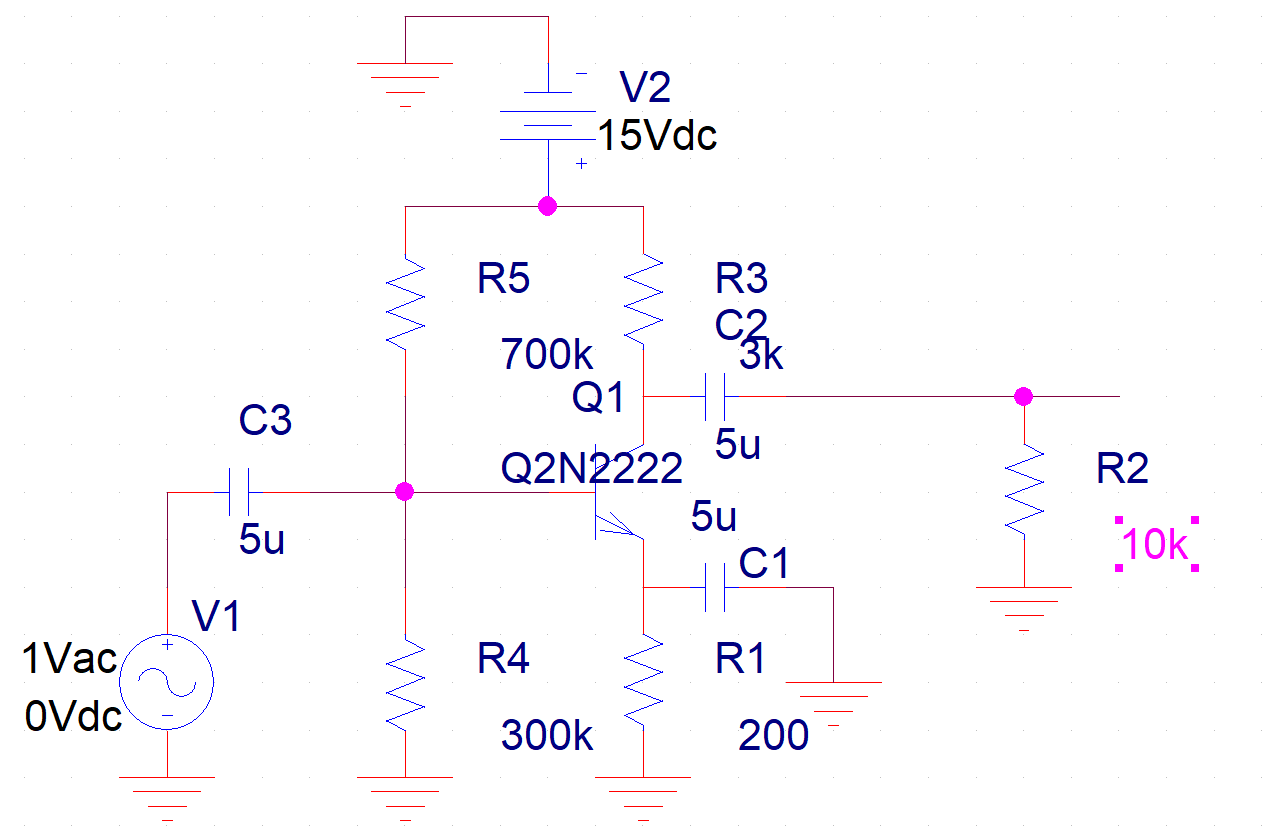
\includegraphics[width=.7\textwidth]{Figures/HW7-3Schem}
      \caption{Circuit Schematic}
      \label{fig:6}
    \end{figure}

    \begin{enumerate}

      \item From here, we can run a DC bias point simulation to obtain:

        \begin{figure}[H]
          \centering
          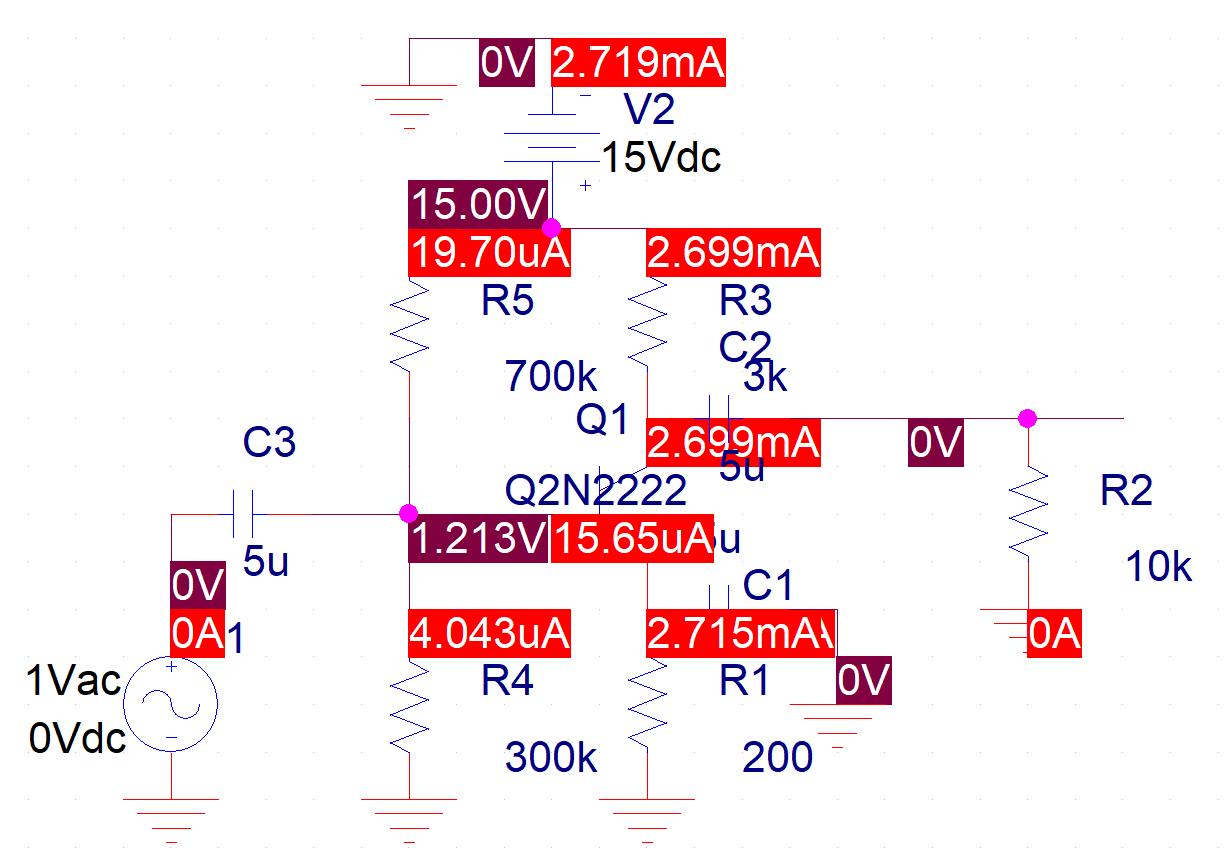
\includegraphics[width=.7\textwidth]{Figures/HW7-3a}
          \caption{Bias Point Simulation Results}
          \label{fig:7}
        \end{figure}

        From the above, we may observe that the voltage at the collector may be written as:

        $$V_{CE}=15-(3)(2.699)$$
        $$V_{CE}=6.903[\si{\volt}]$$

        The base voltage may be observed to be $1.213[\si{\volt}]$. Therefore, because $V_{CE}>V_{BE}$, the BJT is operating in its active mode. Checking the output file, we may find:

        \begin{figure}[H]
          \centering
          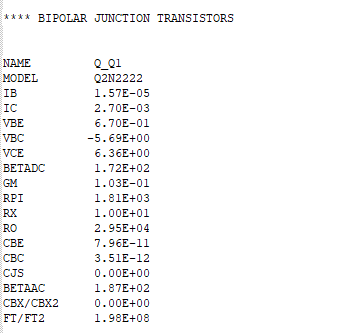
\includegraphics[width=.5\textwidth]{Figures/HW7-3a2}
          \caption{Operating Point Information}
          \label{fig:8}
        \end{figure}

      \item Running an AC Simulation, we obtain the following:

        \begin{figure}[H]
          \centering
          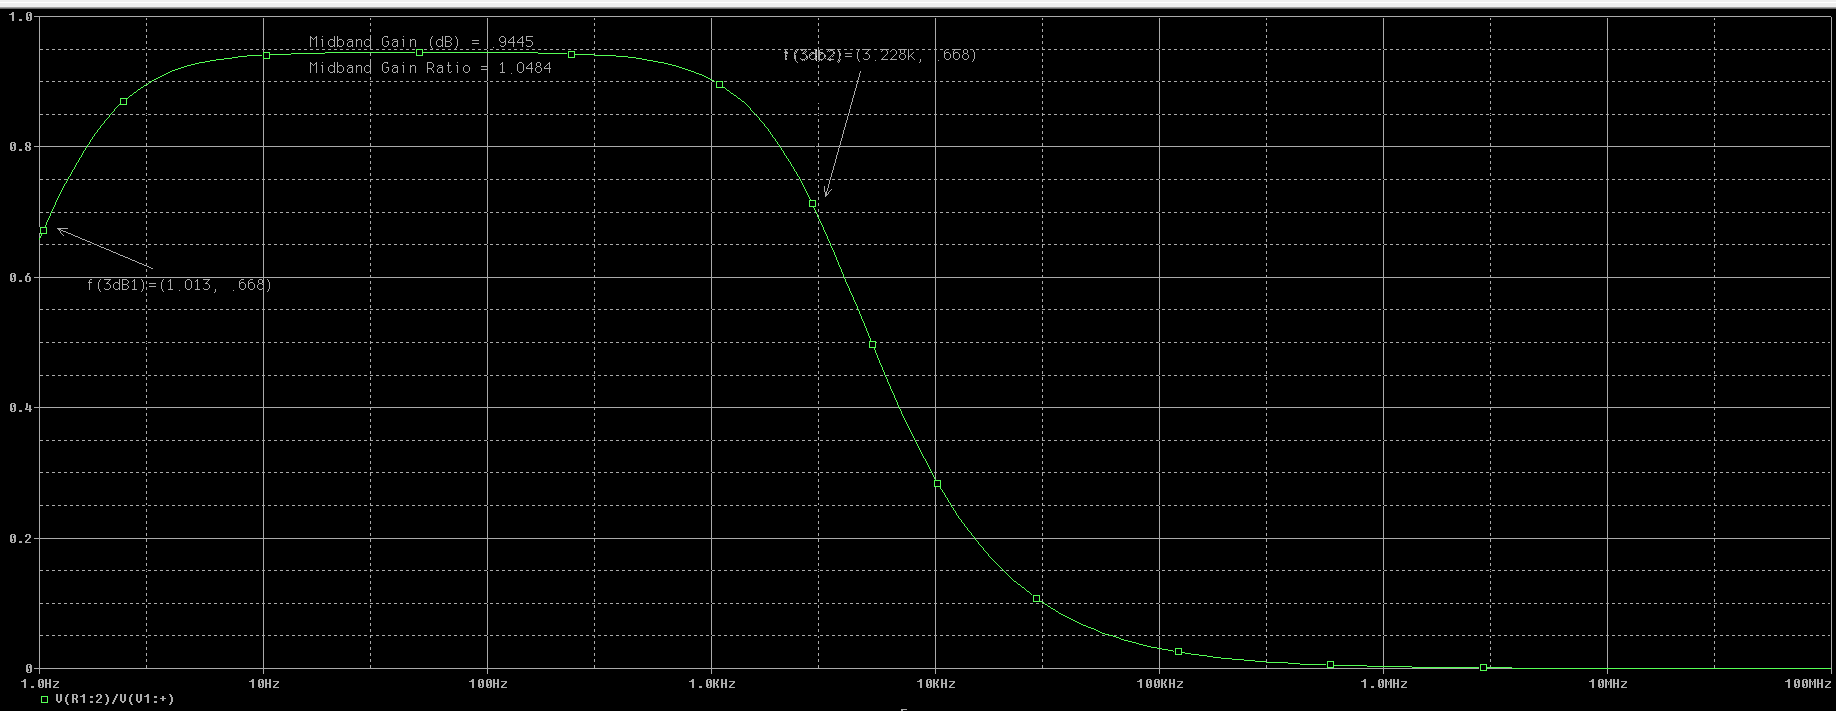
\includegraphics[width=.9\textwidth]{Figures/HW7-3b}
          \caption{AC Simulation, $1[\si{\hertz}]-100[\si{\mega\hertz}]$, 20 Points per Decade}
          \label{fig:9}
        \end{figure}

        The critical values for this circuit are (roughly):

        $$\left\{\begin{array}{ll}\text{Midband Gain: }&46.9[\text{dB}]\\A_v, &218.896\\\text{Low Corner: }&3.2374[\si{\kilo\hertz}]\\\text{High Corner: }& 10.15[\si{\mega\hertz}]\end{array}$$

      \item Running a transient simulation produces the following:

        \begin{figure}[H]
          \centering
          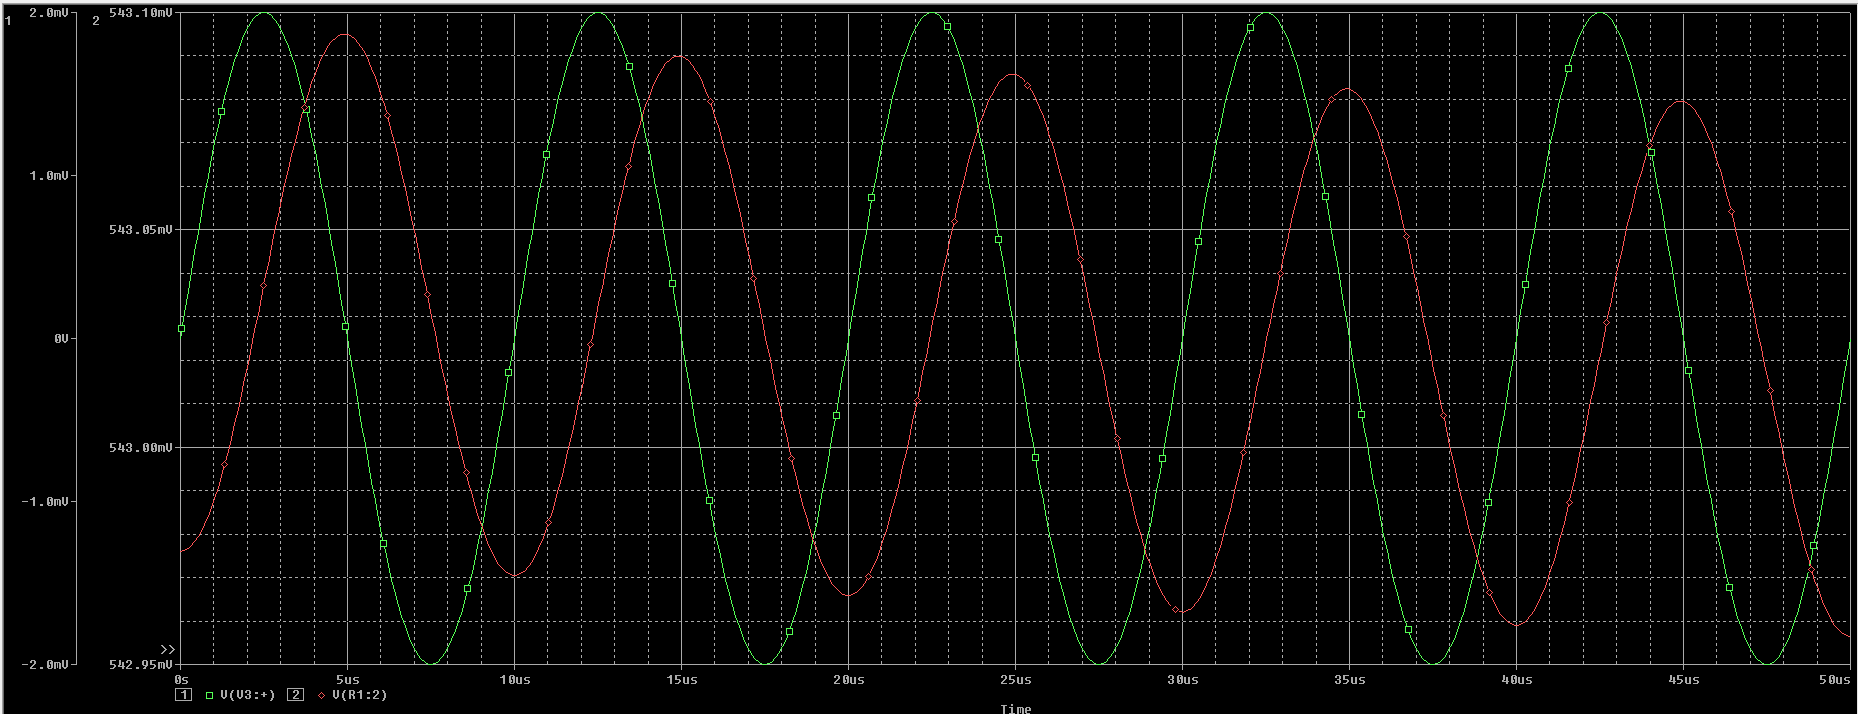
\includegraphics[width=.9\textwidth]{Figures/HW7-3c}
          \caption{Transient Simulation, Sinusoidal Input ($100[\si{\kilo\hertz}]$, $2[\si{\milli\volt}]$), $.1[\si{\micro\second}]$ Step}
          \label{fig:10}
        \end{figure}

        We may calculate the gain as follows, using the peak output voltage over the peak input voltage, and inverted as a result of the inverting amplifier:

        $$A_v=-\frac{437.724}{2}$$
        $$\boxed{A_v=-218.86}$$

        This is close to the value expected from part (b) above.

      \item We now repeat the transient simulation; however, the input voltage now has a peak amplitude of $20[\si{\milli\volt}]$. This produces:

        \begin{figure}[H]
          \centering
          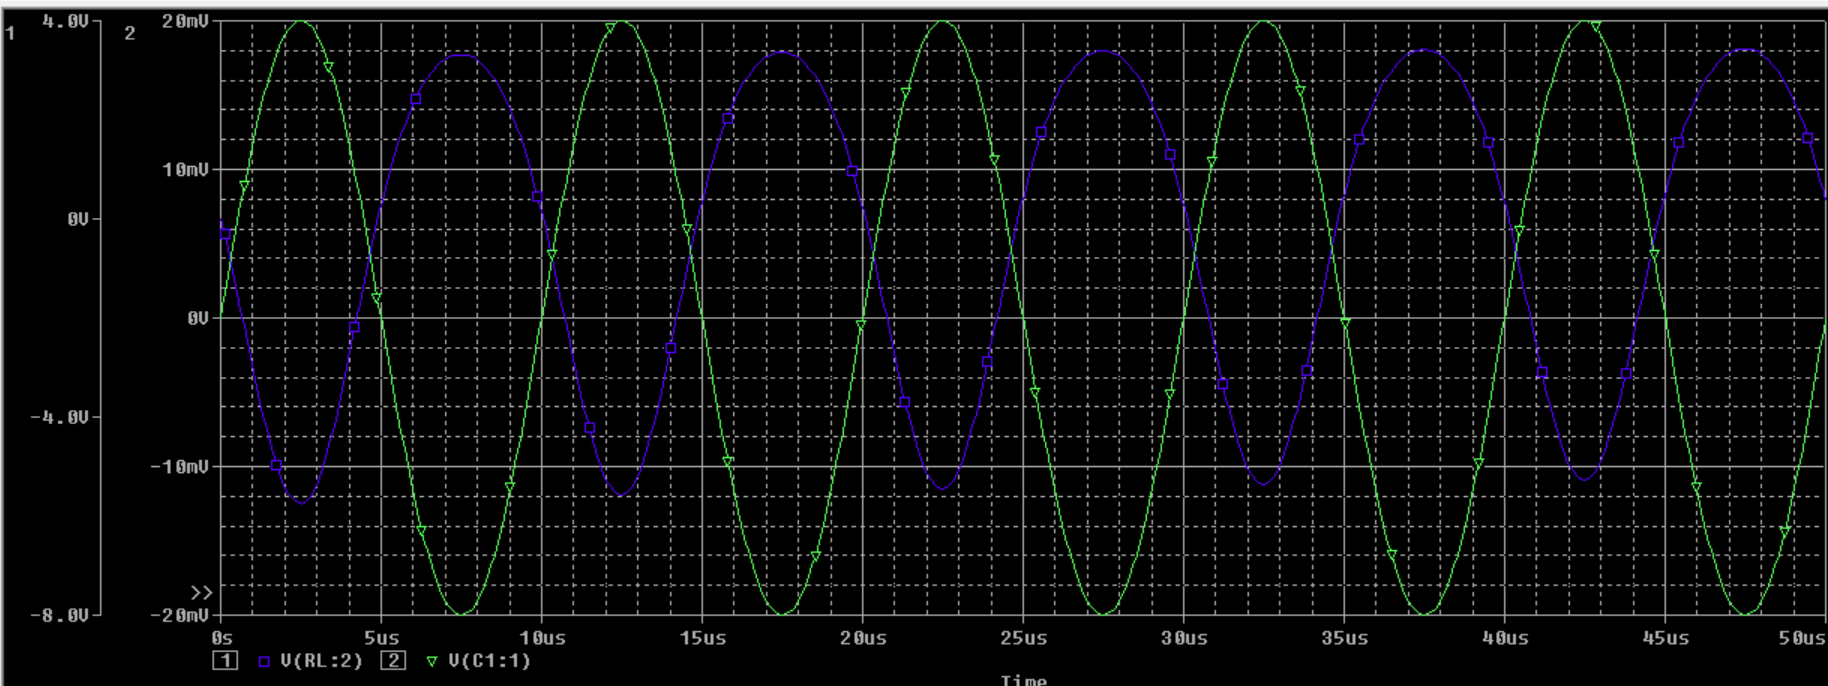
\includegraphics[width=.9\textwidth]{Figures/HW7-3d}
          \caption{Transient Simulation, Sinusoidal Input ($100[\si{\kilo\hertz}]$, $20[\si{\milli\volt}]$), $.1[\si{\micro\second}]$ Step}
          \label{fig:11}
        \end{figure}

        We may observe that, indeed, the output voltage becomes distorted. This is because the $C_3$ capacitor linearizes the amplification, and removing it allows the amplifiers inherent nonlinearities to evince.

      \item Finally, we run both an AC and transient simulation on the circuit with $C_3$ removed. This produces:

        \begin{figure}[H]
          \centering
          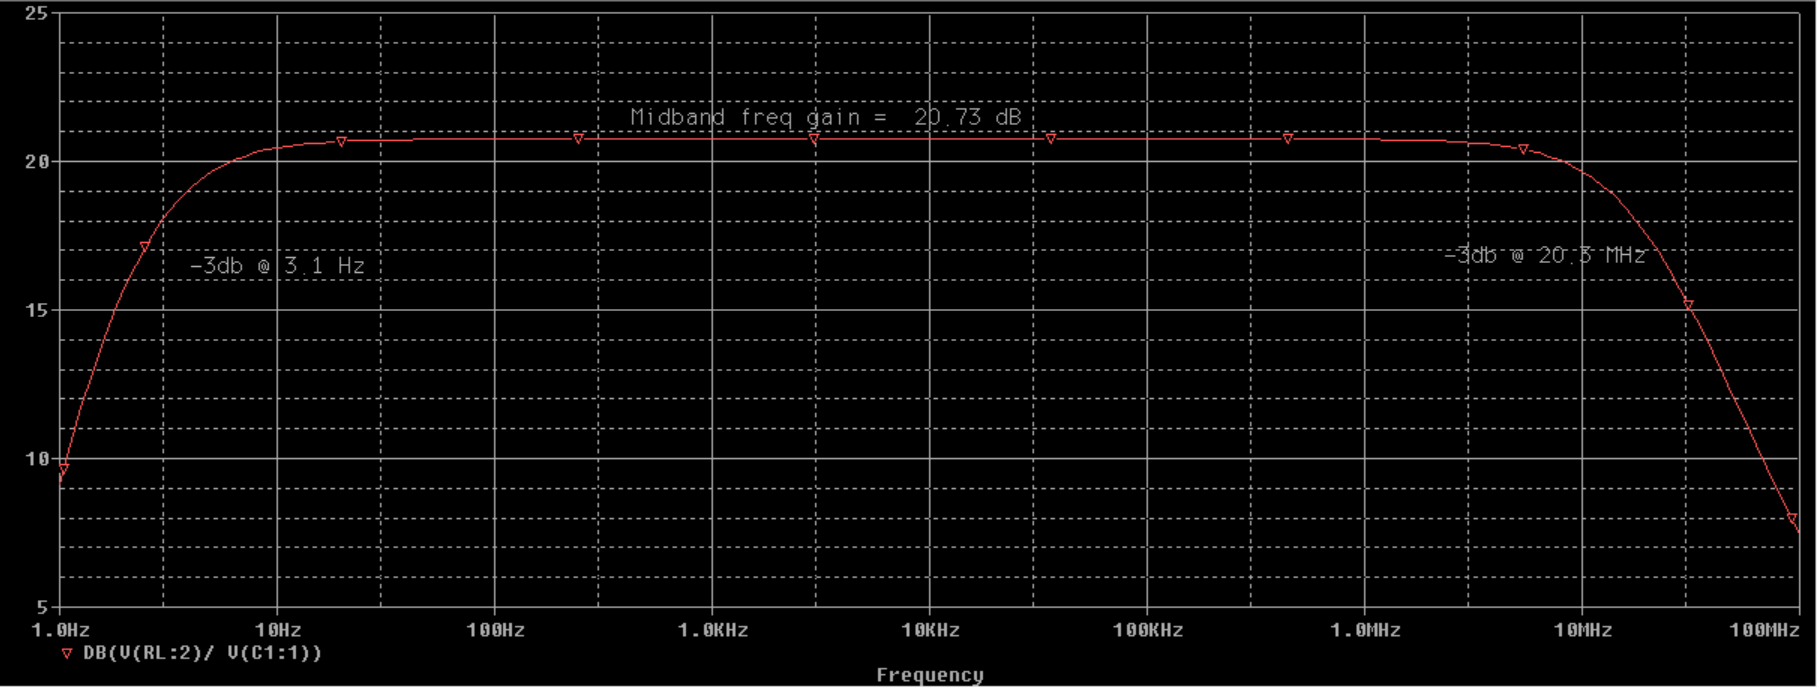
\includegraphics[width=.9\textwidth]{Figures/HW7-3e1}
          \caption{AC Simulation, Same Parameters as Above, No $C_3$ Capacitor}
          \label{fig:12}
        \end{figure}

        \begin{figure}[H]
          \centering
          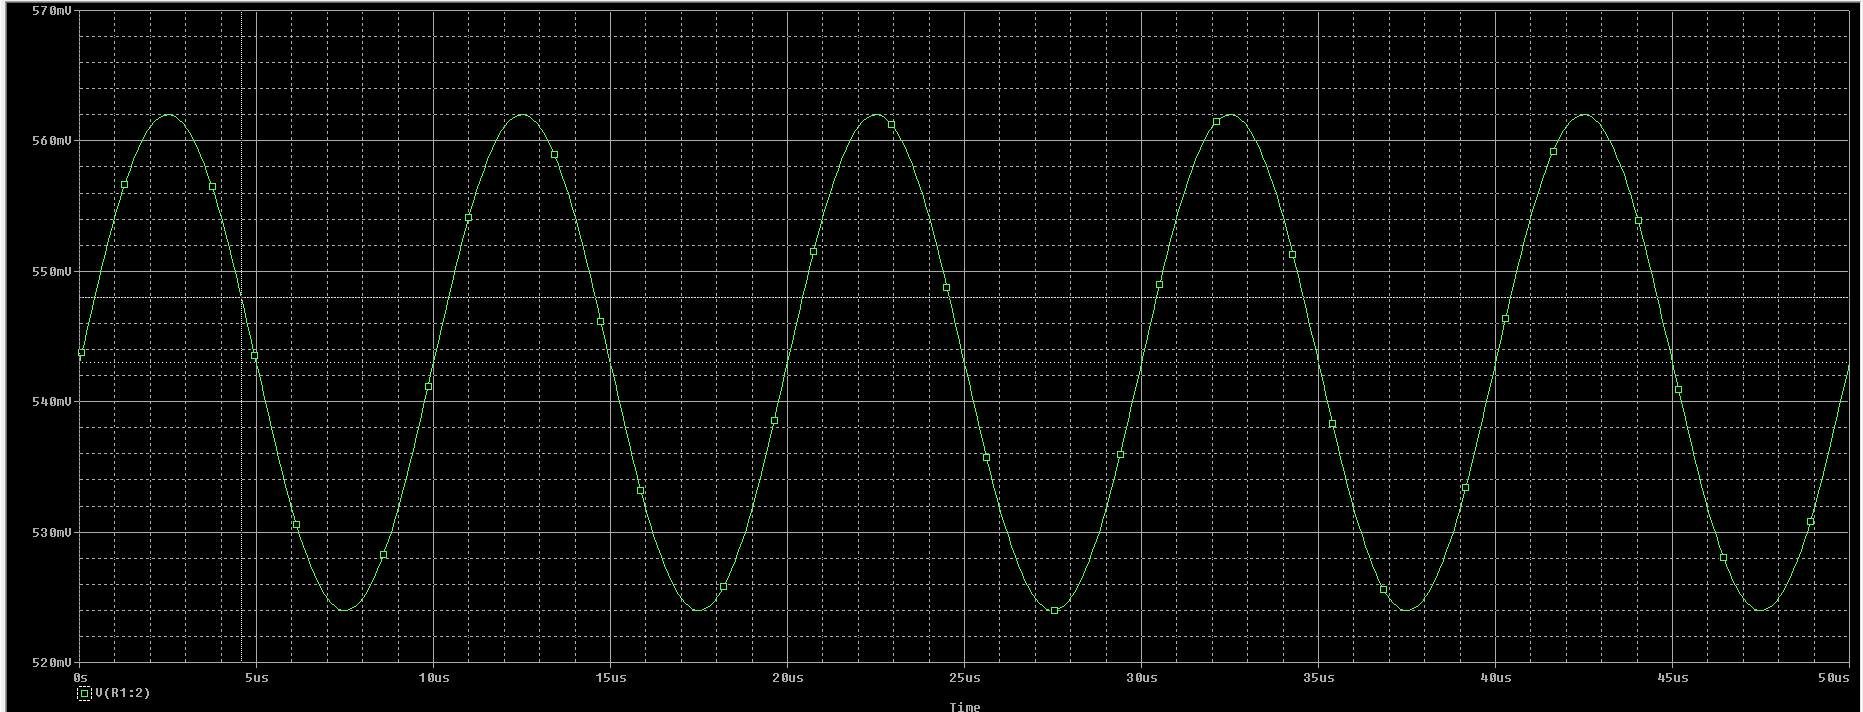
\includegraphics[width=.9\textwidth]{Figures/HW7-3e2}
          \caption{Transient Simulation, Same $20[\si{\milli\volt}]$ Parameters as Above, No $C_3$ Capacitor}
          \label{fig:13}
        \end{figure}

        Based on the output from above, we may conclude that the gain is (based on a \underline{peak voltage} of $217.745[\si{\milli\volt}]$):

        $$\boxed{A_v=-\frac{217.745}{20}=10.887}$$

    \end{enumerate}

\end{enumerate}

\end{document}

